% ============================================================
\section{Architektura počítače, reprezentace čísel, dat a programů}
% ============================================================

Požadavky chtějí umět popsat základní stavbu počítače a hlavně \emph{reprezentaci a~přístup k~datům v~paměti}: jak vypadá adresa a~adresový prostor, jak jsou v~paměti uloženy jednoduché i~složené datové typy a~jak nad nimi pracují základní aritmetické a~logické operace. Tato sekce zavádí pojmy, na kterých staví celý zbytek okruhu (adresy a~offsety u~stránkování, hexdumpy u~obsluhy zařízení, zarovnání u~správce paměti).

\subsection{Základní architektura počítače}

\begin{definice}[Von Neumannova vs. harvardská architektura]
\emph{Von Neumannova architektura} ukládá program i~data do \emph{téže} paměti, přístupné po jedné sběrnici. \emph{Harvardská architektura} má oddělené paměti (a~sběrnice) pro instrukce a~pro data. Běžné PC jsou von Neumannova; harvardská se používá v~mikrokontrolérech a~uvnitř procesoru na úrovni cache (oddělené L1 pro instrukce a~data).
\end{definice}

Procesor (CPU) je stroj, který opakovaně vykonává jednoduché \emph{instrukce}. Adresu právě prováděné instrukce drží registr \emph{IP} (instruction pointer, též PC, program counter).

\begin{definice}[Instrukční cyklus]
Vykonání jedné instrukce probíhá v~krocích: \emph{načti} instrukci z~adresy v~IP (fetch), \emph{dekóduj} ji (decode), \emph{načti operandy}, \emph{proveď} operaci (execute), \emph{ulož} výsledek a~\emph{posuň} IP na následující instrukci. U~některých instrukcí se některé kroky vynechají.
\end{definice}

\begin{intuice}
Celý výpočet je posloupnost těchto cyklů. Procesor sám o~sobě „nerozumí`` cyklům ani funkcím vyššího jazyka -- ty se na instrukce teprve překládají (sekce~2). Význam má jen aktuální obsah registrů a~paměti a~adresa v~IP.
\end{intuice}

\subsection{Paměť, adresa a adresový prostor}

\begin{definice}[Paměť, bajt, adresa, adresový prostor]
Paměť je tvořena \emph{buňkami} (bity) sdruženými do \emph{slov} pevné délky. Dnes je jednotkou adresace \emph{bajt} (byte, 8~bitů): každý bajt má vlastní \emph{adresu}, což je $N$-bitové číslo (typicky $N=32$ nebo $64$). Množina všech adres $[0,\,2^{N})$ je \emph{adresový prostor}; lze v~něm adresovat $2^{N}$ bajtů. Hodnota uložená v~ukazateli (pointeru) je právě taková adresa.
\end{definice}

Jednoduchá data (celé číslo, znak, ukazatel) zabírají souvislou skupinu bajtů začínající na nějaké adrese. U~vícebajtových hodnot je ale nutné dohodnout \emph{pořadí bajtů} v~paměti.

\begin{definice}[Endianita (pořadí bajtů)]
\emph{Little-endian}: na nejnižší adresu se uloží nejméně významný bajt (LSB), na nejvyšší nejvýznamnější (MSB). \emph{Big-endian}: opačně, na nejnižší adresu nejvýznamnější bajt. Intel x86 je little-endian; síťové protokoly TCP/IP používají big-endian (proto „network byte order``).
\end{definice}

\begin{center}
\scalebox{1.25}{%
\begin{tikzpicture}
% hodnota 0x0A0B0C0D ulozena na adresach A..A+3
\foreach \i/\addr in {0/A,1/{A+1},2/{A+2},3/{A+3}} {
  \node[font=\scriptsize\ttfamily] at (\i*0.95+0.475, 1.95) {\addr};
}
% big endian (MSB first)
\node[anchor=east,font=\small] at (-0.15,1.3) {big-endian:};
\foreach \i/\b in {0/0A,1/0B,2/0C,3/0D}
  \node[bunka,minimum width=0.95cm] at (\i*0.95,1.0) {\b};
% little endian (LSB first)
\node[anchor=east,font=\small] at (-0.15,0.3) {little-endian:};
\foreach \i/\b in {0/0D,1/0C,2/0B,3/0A}
  \node[bunka,minimum width=0.95cm] at (\i*0.95,0.0) {\b};
\node[anchor=west,font=\scriptsize] at (4.0,1.35) {MSB na nejnižší adrese};
\node[anchor=west,font=\scriptsize] at (4.0,0.35) {LSB na nejnižší adrese};
\end{tikzpicture}}%
\obrpopis{Uložení 32-bitové hodnoty \texttt{0x0A0B0C0D} od adresy $A$. Bajty hodnoty jsou (od nejvýznamnějšího) \texttt{0A\,0B\,0C\,0D}; liší se jen jejich pořadí v~paměti. Čtení čísla zpět musí použít stejnou konvenci, jakou bylo zapsáno.}
\end{center}

\subsection{Reprezentace celých čísel}

\begin{definice}[Bez znaménka a dvojkový doplněk]
$N$-bitové \emph{číslo bez znaménka} (unsigned) je prostý dvojkový zápis; rozsah je $[0,\,2^{N}-1]$. \emph{Číslo se znaménkem} se ukládá ve \emph{dvojkovém doplňku}: nejvyšší bit má váhu $-2^{N-1}$, ostatní kladné váhy. Rozsah je $[-2^{N-1},\,2^{N-1}-1]$ (asymetrický). Opačnou hodnotu získáme bitovou negací a~přičtením jedničky: $-x=\mathord{\sim}x+1$.
\end{definice}

\begin{intuice}
Dvojkový doplněk má jen \emph{jednu} nulu (na rozdíl od reprezentace „znaménko + velikost``) a~hlavně se sčítá a~odčítá \emph{stejným} obvodem jako čísla bez znaménka -- bity výsledku jsou identické, liší se jen jejich interpretace. Proto má procesor jednu sčítačku pro obě varianty. Např. v~8~bitech je $\texttt{0xFF}=255$ bez znaménka, ale $-1$ se znaménkem; $\texttt{0x80}=128$ resp. $-128$.
\end{intuice}

\subsection{Reprezentace reálných čísel (IEEE 754)}

Reálná čísla se ukládají v~\emph{pohyblivé řádové čárce} (floating point) podle normy IEEE~754. Jednoduchá přesnost (\cd!float!, 32~bitů) má 1~bit znaménka, 8~bitů exponentu a~23~bitů mantisy (zlomkové části).

\begin{center}
\scalebox{1.2}{%
\begin{tikzpicture}
% bitove pole: 1 + 8 + 23
\node[bit,minimum width=0.7cm,fill=red!12] (s) at (0,0) {$s$};
\node[bit,minimum width=2.4cm,fill=blue!10] (e) at (0.7,0) {exponent $e$ (8~b)};
\node[bit,minimum width=4.6cm,fill=green!10] (m) at (3.1,0) {mantisa $f$ (23~b)};
% bitove indexy
\node[font=\scriptsize,anchor=south] at (0.35,0.7) {31};
\node[font=\scriptsize,anchor=south] at (1.9,0.7) {30\,$\ldots$\,23};
\node[font=\scriptsize,anchor=south] at (5.4,0.7) {22\,$\ldots$\,0};
\end{tikzpicture}}%
\obrpopis{Formát IEEE~754 single (32~b). Hodnota normalizovaného čísla je $(-1)^{s}\cdot(1{.}f)_2\cdot 2^{\,e-127}$, kde exponent je uložen s~posunem (bias) $127$ a~před mantisou se předpokládá implicitní jednička. Např. $1{.}0=(-1)^0\cdot1{.}0\cdot2^{127-127}$, tj. $s{=}0$, $e{=}127{=}\texttt{0x7F}$, $f{=}0$, dohromady \texttt{0x3F800000}.}
\end{center}

\begin{poznamka}
Krajní hodnoty exponentu jsou vyhrazené: samé nuly kódují nulu a~\emph{denormalizovaná} čísla (velmi malá), samé jedničky kódují $\pm\infty$ (mantisa~0) a~\emph{NaN} (mantisa~$\neq0$). Dvojitá přesnost (\cd!double!, 64~b) má stejnou strukturu s~11~bity exponentu a~52~bity mantisy.
\end{poznamka}

\subsection{Základní aritmetické a logické operace}

Procesor poskytuje \emph{aritmetické} instrukce ($+$, $-$, $\times$, celočíselné $/$ a~zbytek $\%$) a~\emph{bitové/logické} instrukce: bitové \emph{a}~(\cd!&!), \emph{nebo}~(\cd!|!), \emph{xor}~(\cd!^!), negace~(\cd!~!) a~\emph{posuny}.

\begin{definice}[Posuny a přetečení]
\emph{Logický posun} (\cd!<<!, \cd!>>! na unsigned) doplňuje nuly; \emph{aritmetický posun vpravo} (na signed) doplňuje znaménkový bit, takže zachová znaménko. Posun vlevo o~$k$ je násobení $2^{k}$, posun vpravo dělení $2^{k}$ (dolů). \emph{Přetečení} (overflow): u~čísel bez znaménka výsledek „přeteče`` modulo $2^{N}$; u~znaménkových je přetečení, když pravý matematický výsledek leží mimo rozsah dvojkového doplňku.
\end{definice}

\subsection{Ukládání složených typů a zarovnání}

Složené typy (struktury, pole) jsou poskládané z~jednodušších, ale ne libovolně těsně.

\begin{definice}[Zarovnání a výplň (padding)]
\emph{Zarovnání} (alignment) datového typu velikosti $s$ znamená, že jeho adresa musí být dělitelná $s$ (procesory to pro efektivní přístup vyžadují, příp.\ silně preferují). Struktura se zarovnává podle svého \emph{největšího} členu. Aby každý člen padl na svou zarovnanou adresu, vkládá překladač mezi členy nevyužité bajty -- \emph{vnitřní výplň} (inner padding) -- a~na konec struktury \emph{vnější výplň} (outer padding) tak, aby i~v~poli za sebou jdoucí prvky zůstaly zarovnané, tj. velikost struktury je násobkem jejího zarovnání.
\end{definice}

\begin{center}
\scalebox{1.15}{%
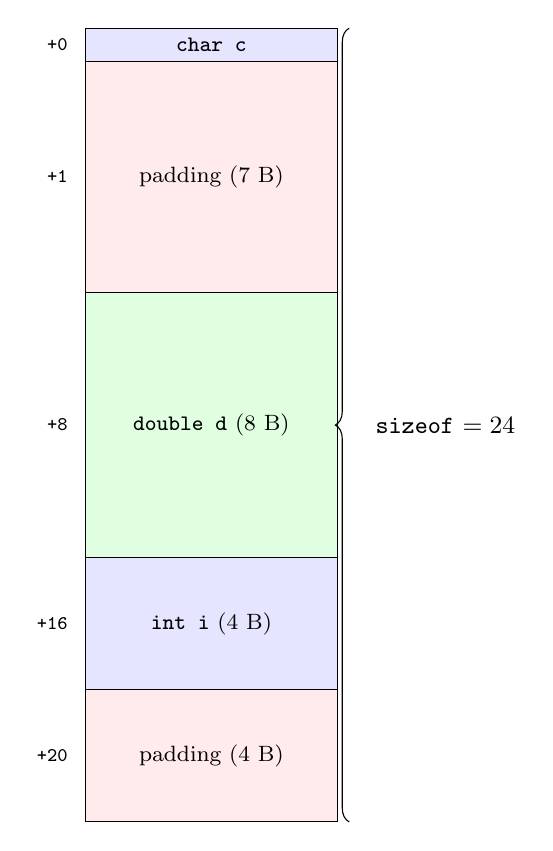
\begin{tikzpicture}[y=0.42cm,every node/.append style={font=\footnotesize}]
% struct dem { char c; double d; int i; } na 64-bit, zarovnani 8; y-jednotka = 1 bajt
% poradi zdola nahoru = od nejvyssich offsetu (dole) k offsetu 0 (nahore)
\fill[red!8]   (0,0)  rectangle (3.2,4);   \draw (0,0)  rectangle (3.2,4);
\fill[blue!10] (0,4)  rectangle (3.2,8);   \draw (0,4)  rectangle (3.2,8);
\fill[green!12](0,8)  rectangle (3.2,16);  \draw (0,8)  rectangle (3.2,16);
\fill[red!8]   (0,16) rectangle (3.2,23);  \draw (0,16) rectangle (3.2,23);
\fill[blue!10] (0,23) rectangle (3.2,24);  \draw (0,23) rectangle (3.2,24);
\node at (1.6,2)    {padding (4~B)};
\node at (1.6,6)    {\texttt{int i} (4~B)};
\node at (1.6,12)   {\texttt{double d} (8~B)};
\node at (1.6,19.5) {padding (7~B)};
\node at (1.6,23.5) {\texttt{char c}};
\node[anchor=east,font=\scriptsize\ttfamily] at (-0.1,2)    {+20};
\node[anchor=east,font=\scriptsize\ttfamily] at (-0.1,6)    {+16};
\node[anchor=east,font=\scriptsize\ttfamily] at (-0.1,12)   {+8};
\node[anchor=east,font=\scriptsize\ttfamily] at (-0.1,19.5) {+1};
\node[anchor=east,font=\scriptsize\ttfamily] at (-0.1,23.5) {+0};
\draw[decorate,decoration={brace,amplitude=5pt}] (3.35,0) -- (3.35,24)
  node[midway,anchor=west,xshift=6pt,font=\small] {\texttt{sizeof} $=24$};
\end{tikzpicture}}%
\obrpopis{Rozložení \texttt{struct \{ char c; double d; int i; \}} v~paměti (64-bit, zarovnání struktury $=8$ podle \texttt{double}). \texttt{c} je na offsetu $0$, ale \texttt{d} musí začínat na násobku~$8$, proto je za \texttt{c} vnitřní výplň $7$~B. Za \texttt{i} (offsety $16$--$19$) je vnější výplň $4$~B, aby celková velikost $24$ byla násobkem~$8$. Holá data zabírají $1{+}8{+}4=13$~B, struktura ale $24$~B.}
\end{center}

\subsection{Řešený příklad: reprezentace dat v binárním souboru}

\begin{priklad}[SZZ podzim 2025 č.~2: Reprezentace dat v binárním souboru]
\szzotazka{podzim 2025}{2}{Ukládání dat v binárním souboru (hexdump, reprezentace dat)}\par
\textbf{Zadání.}\par
Soubor ukládá \emph{uzly} se stejnou sadou \emph{atributů}. Hlavička na začátku obsahuje 2~bajty s~počtem atributů, pak po jednom bajtu typ každého atributu (\cd!enum AttrType { TUInt16=0x48, TLink=0x4C, TString=0x53, TSInt16=0x68 }!). Vícebajtová čísla jsou \textbf{big-endian}. Hned za hlavičkou je kořenový uzel: 2~bajty délky dat, pak hodnoty atributů. \texttt{TUInt16}/\texttt{TSInt16} jsou 2~bajty (bez/se znaménkem, dvojkový doplněk), \texttt{TString} je 2~bajty délky $+$ ASCII znaky, \texttt{TLink} je 8~bajtů (pozice jiného uzlu). Třída \texttt{BinaryFile} nabízí \cd!void readBytes(long filepos, byte[] buf, int len)!. Úkolem je napsat třídu \texttt{Reader} (konstruktor načte hlavičku; \texttt{attributes}, \texttt{getType}, \texttt{getRoot}, \texttt{readNode}) a~třídu \texttt{Node} (data jako pole bajtů $+$ struktura pro lokalizaci atributu v~konstantním čase; metody \texttt{getUInt16}, \texttt{getSInt16}).

\medskip
\textbf{Řešení.}\par
\textbf{(1)~Dekódování ukázkového hexdumpu.} Nejdřív si rozmysleme, jak se daný výpis čte -- to je jádro úlohy. Bajty jsou (offsety vlevo):
\begin{lstlisting}
0000:  00 06  48 68 53 53 4C 4C   <- hlavicka: 0x0006 = 6 atributu, pak typy
0008:  00 22  03 E8  FC 18  ...   <- korenovy uzel: 0x0022 = 34 B dat
\end{lstlisting}
Typy atributů jsou \texttt{0x48,0x68,0x53,0x53,0x4C,0x4C}, tj. \texttt{TUInt16, TSInt16, TString, TString, TLink, TLink}. Kořenový uzel začíná na offsetu~8 (za 2~B počtu a~6~B typů); jeho data (34~B) se čtou podle typů:
\begin{enumerate}
\item \texttt{TUInt16}: \texttt{03 E8} big-endian $=\texttt{0x03E8}=\boxed{1000}$.
\item \texttt{TSInt16}: \texttt{FC 18} $=\texttt{0xFC18}$; nejvyšší bit~1, tedy záporné: $\texttt{0xFC18}-2^{16}=\boxed{-1000}$.
\item \texttt{TString}: délka \texttt{00 05} $=5$, pak \texttt{48 65 6C 6C 6F} $=\boxed{\text{\texttt{"Hello"}}}$.
\item \texttt{TString}: délka \texttt{00 05} $=5$, pak \texttt{57 6F 72 6C 64} $=\boxed{\text{\texttt{"World"}}}$.
\item \texttt{TLink}: 8~bajtů \texttt{00\,00\,00\,00\,00\,00\,00\,2C} $=\boxed{\texttt{0x2C}}$.
\item \texttt{TLink}: 8~bajtů \texttt{00\,00\,00\,00\,00\,00\,12\,34} $=\boxed{\texttt{0x1234}}$.
\end{enumerate}
Spotřebovaná délka je $2+2+(2{+}5)+(2{+}5)+8+8=34$~B, což přesně sedí s~deklarovanou délkou uzlu.

\medskip
\textbf{(2)~Třída \texttt{Reader}.} Konstruktor přečte počet atributů a~jejich typy; \texttt{getRoot} vrací offset hned za hlavičkou. \texttt{readNode} přečte 2~bajty délky a~pak \texttt{len} bajtů dat. Pomocné big-endian čtení 16-bit čísla:
\begin{lstlisting}[language=C++]
struct Reader {
  BinaryFile& f;  int nattr;  std::vector<unsigned char> types;
  Reader(BinaryFile& bf) : f(bf) {
    unsigned char h[2];  f.readBytes(0, h, 2);
    nattr = (h[0] << 8) | h[1];            // big-endian
    types.resize(nattr);  f.readBytes(2, types.data(), nattr);
  }
  int attributes()      { return nattr; }
  int getType(int i)    { return types[i]; }
  long getRoot()        { return 2 + nattr; }     // hned za hlavickou
  Node readNode(long filepos) {
    unsigned char len2[2];  f.readBytes(filepos, len2, 2);
    int len = (len2[0] << 8) | len2[1];
    std::vector<unsigned char> data(len);
    f.readBytes(filepos + 2, data.data(), len);
    return Node(types, std::move(data));
  }
};
\end{lstlisting}

\textbf{(3)~Třída \texttt{Node}.} Data drží jako pole bajtů; aby šel $i$-tý atribut najít v~$O(1)$, předpočítá v~konstruktoru pole \emph{offsetů} každého atributu uvnitř dat (řetězce mají proměnnou délku, proto se offsety musí jednou projít). Převod na číslo dělají \texttt{get} metody pomocí big-endian skládání:
\begin{lstlisting}[language=C++]
struct Node {
  std::vector<unsigned char> data;  std::vector<int> off;   // off[i] = pozice atributu i
  Node(const std::vector<unsigned char>& types, std::vector<unsigned char> d)
      : data(std::move(d)) {
    int p = 0;
    for (unsigned char t : types) {
      off.push_back(p);
      if (t == 0x48 || t == 0x68) p += 2;                    // TUInt16 / TSInt16
      else if (t == 0x4C)         p += 8;                    // TLink
      else if (t == 0x53)         p += 2 + ((data[p]<<8)|data[p+1]);  // TString
    }
  }
  int getUInt16(int i) { int p=off[i]; return (data[p]<<8) | data[p+1]; }
  int getSInt16(int i) { int v=getUInt16(i); return v>=0x8000 ? v-0x10000 : v; }
};
\end{lstlisting}
\textit{Pozn.: V~PDF tato otázka náčrt řešení nemá; dekódování i~kód jsme ověřili skriptem \texttt{verify\_szz.py} (hodnoty \texttt{\{1000, -1000, "Hello", "World", 0x2C, 0x1234\}}).}
\end{priklad}

\subsection{Dynamická správa paměti na haldě}

Lokální proměnné a~argumenty žijí na \emph{zásobníku} (alokace posunem ukazatele, sekce~2), globální mají pevné místo. Proměnné, jejichž životnost neurčuje rozsah bloku, se alokují dynamicky na \emph{haldě} (heap): běhové prostředí (resp.\ OS) spravuje velký blok paměti a~přiděluje z~něj kusy na žádost.

\begin{intuice}
Dynamická alokace není v~doslovných požadavcích okruhu, ale objevuje se v~SZZ otázce léto~2025 a~přesně procvičuje reprezentaci dat v~paměti, zarovnání a~práci s~adresami a~offsety -- proto ji řešíme jako příklad. Správce vede \emph{evidenci volných bloků} (typicky vázaný seznam) a~na žádost vybere vhodný blok strategií \emph{first-fit} (první dost velký od začátku), případně best/next/worst-fit. Volné místo se časem tříští (\emph{fragmentace}).
\end{intuice}

\begin{priklad}[SZZ léto 2025 č.~2: Jednoduchý správce paměti]
\szzotazka{léto 2025}{2}{Jednoduchý správce paměti (heap alokátor, 32-bit)}\par
\textbf{Zadání.}\par
V~souvislém poli bajtů (little-endian) implementujeme heap. Každý \emph{podblok} je zarovnaný na 2~bajty a~má 16-bitovou hlavičku \texttt{Size} na offsetu \texttt{+0} = velikost podbloku \emph{včetně hlavičky}. Protože velikost je sudá, je její bit~0 vždy~0 a~používá se jako příznak: $0=$ volný, $1=$ obsazený. Volný podblok má navíc na \texttt{+2} položku \texttt{Next} (16-bit offset dalšího volného podbloku, $-1=\texttt{0xFFFF}$ u~posledního), zbytek je vynulovaný; volné podbloky tak tvoří jednosměrný seznam. Obsazený podblok má na \texttt{+2} rovnou payload. Pamatujeme si offset prvního volného podbloku; na počátku je heap jeden volný podblok velikosti celého heapu. Alokuje se strategií \emph{first-fit}. Dány metody \cd!SetUshort!/\cd!GetUshort! (čtení/zápis 16-bit hodnoty little-endian). Úkoly: (1)~konstruktor, (2)~\texttt{FindFirstFree}, (3)~\texttt{Mark}, (4)~hexdump 22~B heapu po \cd!A=Alloc(2); B=Alloc(4); C=Alloc(2); Free(B)!.

\medskip
\textbf{Řešení.}\par
\textbf{(1)--(3)~Metody.} Potřebná velikost podbloku je payload~$+\,2$~(hlavička), zaokrouhleno na sudé číslo. Konstruktor založí jediný volný podblok přes celý heap (a~podle zadání vynuluje jeho zbytek, paměť nemusí přijít vynulovaná); \texttt{FindFirstFree} projde seznam volných a~vrátí první dost velký; \texttt{Mark} jen přepíše bit~0 položky \texttt{Size}.
\begin{lstlisting}[language={[Sharp]C}]
public Heap(byte[] availableMemory) {
    _heap = availableMemory;
    _firstFreeOffset = 0;
    SetUshort(0, (ushort)_heap.Length);   // Size = cely heap, bit0=0 (volny)
    SetUshort(2, 0xFFFF);                  // Next = -1 (posledni volny)
    for (int i = 4; i < _heap.Length; i++) // zbytek volneho podbloku nulovy
        _heap[i] = 0;
}
private ushort FindFirstFree(ushort payloadSize) {
    ushort need = (ushort)(payloadSize + 2);
    if ((need & 1) != 0) need++;                       // zarovnani na 2
    ushort o = _firstFreeOffset;
    while (o != 0xFFFF) {
        ushort size = (ushort)(GetUshort(o) & 0xFFFE); // bit0 je priznak
        if (size >= need) return o;
        o = GetUshort((ushort)(o + 2));                // Next
    }
    return 0xFFFF;                                     // nenalezeno
}
private void Mark(ushort offset, bool isFree) {
    ushort size = GetUshort(offset);
    SetUshort(offset, isFree ? (ushort)(size & 0xFFFE)
                             : (ushort)(size | 1));
}
\end{lstlisting}

\textbf{(4)~Stav heapu krok po kroku} (heap má 22~B, na počátku samé nuly, jeden volný podblok velikosti $22$ s~\texttt{Next}$=-1$):
\begin{enumerate}
\item \cd!Alloc(2)! $\to$ potřeba $2{+}2=4$. First-fit vezme volný blok \texttt{@0} ($22\ge4$), rozdělí: \textbf{A} obsazený \texttt{@0} velikosti~4, zbytek volný \texttt{@4} velikosti~18. Payload~A na \texttt{@2}.
\item \cd!Alloc(4)! $\to$ potřeba $4{+}2=6$. Volný \texttt{@4} ($18\ge6$): \textbf{B} obsazený \texttt{@4} velikosti~6, zbytek volný \texttt{@10} velikosti~12. Payload~B na \texttt{@6}.
\item \cd!Alloc(2)! $\to$ potřeba~4. Volný \texttt{@10} ($12\ge4$): \textbf{C} obsazený \texttt{@10} velikosti~4, zbytek volný \texttt{@14} velikosti~8. Payload~C na \texttt{@12}.
\item \cd!Free(B)!: payload~B byl na \texttt{@6}, podblok tedy \texttt{@4}; označí se volným. Do seznamu volných se vloží podle offsetu: první volný je nyní \texttt{@4} ($\texttt{Next}\to14$), pak \texttt{@14} ($\texttt{Next}=-1$).
\end{enumerate}
Výsledné podbloky: A obsazený \texttt{@0} (Size~5), volný \texttt{@4} (Size~6, Next~14), C obsazený \texttt{@10} (Size~5), volný \texttt{@14} (Size~8, Next~$-1$). Hexdump (16-bit hodnoty little-endian; \texttt{Size} obsazeného je $\text{velikost}\,|\,1$):
\begin{center}\ttfamily\small
\begin{tabular}{r|cccccccc}
offset & +0 & +1 & +2 & +3 & +4 & +5 & +6 & +7\\\hline
0x0000 & 05 & 00 & 00 & 00 & 06 & 00 & 0E & 00\\
0x0008 & 00 & 00 & 05 & 00 & 00 & 00 & 08 & 00\\
0x0010 & FF & FF & 00 & 00 & 00 & 00 & -- & --\\
\end{tabular}
\end{center}

\begin{center}
\scalebox{1.1}{%
\begin{tikzpicture}[x=0.42cm,every node/.append style={font=\footnotesize}]
% x-jednotka = 1 bajt; bloky: @0 A obs.(4), @4 volny(6), @10 C obs.(4), @14 volny(8)
\fill[red!8]   (0,0)  rectangle (4,1);   \draw (0,0)  rectangle (4,1);
\fill[green!10](4,0)  rectangle (10,1);  \draw (4,0)  rectangle (10,1);
\fill[red!8]   (10,0) rectangle (14,1);  \draw (10,0) rectangle (14,1);
\fill[green!10](14,0) rectangle (22,1);  \draw (14,0) rectangle (22,1);
\node at (2,0.66)  {\textbf{A} obs.};  \node at (2,0.3)  {Size 5};
\node at (7,0.66)  {volný};            \node at (7,0.3)  {Size 6};
\node at (12,0.66) {\textbf{C} obs.};  \node at (12,0.3) {Size 5};
\node at (18,0.66) {volný};            \node at (18,0.3) {Size 8};
\foreach \x in {0,4,10,14,22}
  \node[anchor=north,font=\scriptsize\ttfamily] at (\x,-0.05) {\x};
\draw[ptr,blue!60!black] (7,1.05) to[bend left=30] node[above,font=\scriptsize]{Next} (18,1.05);
\node[anchor=east,font=\scriptsize,blue!60!black] at (3.2,1.3) {firstFree};
\draw[ptr,blue!60!black] (3.3,1.28) -- (5,1.06);
\node[anchor=west,font=\scriptsize] at (22.4,1.1) {$\to-1$};
\end{tikzpicture}}%
\obrpopis{Stav heapu po \texttt{Alloc(2)/Alloc(4)/Alloc(2)/Free(B)}. Obsazené podbloky A,~C (červeně) zůstaly, uvolněný B se stal volným podblokem \texttt{@4}. Volné podbloky tvoří seznam \texttt{firstFree}$\to$\texttt{@4}$\to$\texttt{@14}$\to-1$. U~obsazených bloků je v~poli \texttt{Size} nastaven příznakový bit~0, proto se reálná velikost~4 uloží jako \texttt{Size}~$5=4\,|\,1$. Hexdump výše ověřen simulací (\texttt{verify\_szz.py}).}
\end{center}
\end{priklad}
